\documentclass[runningheads]{llncs}

\usepackage{graphicx}
\usepackage{amsmath,amssymb}
\usepackage{booktabs}
\usepackage{multirow}
\usepackage{array}
\usepackage[table]{xcolor}
\usepackage{pifont}
\usepackage{hyperref}
\usepackage{listings}
\usepackage{microtype}
\usepackage{tikz}
\usepackage{pgfplots}
\pgfplotsset{compat=1.18}
\usetikzlibrary{shapes.geometric, arrows.meta, positioning, calc, fit, backgrounds}

% Float spacing optimization for 15-page LNCS budget
\setlength{\textfloatsep}{9pt plus 2pt minus 2pt}
\setlength{\floatsep}{7pt plus 2pt minus 2pt}
\setlength{\intextsep}{7pt plus 2pt minus 2pt}
\setlength{\abovecaptionskip}{4pt}
\setlength{\belowcaptionskip}{3pt}
\setlength{\emergencystretch}{2em}

% Publication color palette
\definecolor{checkgreen}{HTML}{2E7D32}
\definecolor{crossred}{HTML}{C62828}
\definecolor{ourgreen}{HTML}{E8F5E9}
\definecolor{headergray}{HTML}{ECEFF1}
\definecolor{boxgray}{HTML}{F8F9FA}
\definecolor{color_symcode}{HTML}{3867D6}       % Royal Slate Blue
\definecolor{color_symplan}{HTML}{10AC84}       % Vibrant Emerald Green
\definecolor{color_plan}{HTML}{FA8231}          % Warm Sunset Coral
\definecolor{color_contract}{HTML}{8854D0}      % Deep Wisteria Purple
\definecolor{chart_grid}{HTML}{E2E8F0}          % Soft Slate for Grid
\definecolor{chart_text}{HTML}{2D3748}          % Charcoal for Text

\newcommand{\cmark}{\textcolor{checkgreen}{\ding{51}}}
\newcommand{\xmark}{\textcolor{crossred}{\ding{55}}}

\lstdefinestyle{promptstyle}{
  basicstyle=\ttfamily\scriptsize,
  backgroundcolor=\color{boxgray},
  frame=single,
  rulecolor=\color{black!25},
  breaklines=true,
  breakatwhitespace=true,
  columns=fullflexible,
  keepspaces=true,
  xleftmargin=1.5mm,
  xrightmargin=1.5mm
}

\begin{document}

\title{SymPlan: Enhancing Neurosymbolic Mathematical Reasoning in Compact Language Models via Representation and Planning}
\titlerunning{SymPlan: Neurosymbolic Reasoning in SLMs}

% -----------------------------------------------------------------------------
% Double-Blind Submission for AMI 2026 (Springer CCIS Series)
% Author names and affiliations omitted for blind review.
% -----------------------------------------------------------------------------
\author{Anonymous Author(s)}
\authorrunning{Anonymous et al.}
\institute{Paper under double-blind review for AMI 2026}

% -----------------------------------------------------------------------------
% Camera-Ready Author Block (Uncomment for final submission):
% \author{Tay Bui\inst{1,2}\orcidID{0009-0000-0000-0000} \and
% Huy N. G. Pham\inst{1,2}\orcidID{0009-0000-0000-0000} \and
% Nhan Ha Le Thanh\inst{3}\orcidID{0009-0000-0000-0000}}
% \authorrunning{T. Bui et al.}
% \institute{University of Information Technology, Ho Chi Minh City, Vietnam \and
% Vietnam National University, Ho Chi Minh City, Vietnam \and
% FPT University, Ho Chi Minh City, Vietnam\\
% \email{\{24521589, 24520690\}@gm.uit.edu.vn, hnhan5355@gmail.com}}
% -----------------------------------------------------------------------------

\maketitle

\begin{abstract}
Coupling generative language models with external symbolic engines offers a transformative pathway toward verifiable mathematical problem solving by grounding continuous linguistic inference in exact deterministic computation. However, conventional neurosymbolic systems adhere to a monolithic synthesis paradigm, compelling models to concurrently decipher informal problem text, synthesize multi-step algebraic strategies, and negotiate rigid formal library syntax within an unguided generation pass. While scalable frontier backbones absorb this cognitive burden, compact language models suffer acute cognitive overextension, triggering semantic drift, domain boundary omissions, and silent regressions during iterative self-repair. We introduce \textbf{SymPlan}, an inspectable neurosymbolic framework that establishes disciplined structural scaffolding tailored to compact backbones. SymPlan decouples symbolic reasoning into three coordinated abstractions: (1) a \textit{Fused Target-Planning Phase} that jointly formalizes the queried mathematical target, a categorical output contract, and an algorithmic roadmap prior to code synthesis; (2) \textit{Contract-Guided Code Generation} that restricts execution to verified algebraic transformations and explicit domain filters; and (3) \textit{Targeted Debugging with Anti-Regression Selection}, which couples static structural diagnostics with an episodic ranking criterion to safeguard valid intermediate derivations against speculative revisions. Extensive empirical evaluations across diverse open-weight model families demonstrate that structural scaffolding systematically resolves formalization bottlenecks, achieving substantial improvements in execution stability and mathematical accuracy over both monolithic code synthesis and step-by-step natural language reasoning without requiring parameter adaptation.

\keywords{Neurosymbolic Reasoning \and Mathematical Problem Solving \and Small Language Models \and SymPy Code Generation \and Algorithmic Planning.}
\end{abstract}

\section{Introduction}

Large Language Models (LLMs) have demonstrated strong multi-step mathematical reasoning through Chain-of-Thought (CoT) prompting~\cite{wei2022cot} and iterative self-consistency sampling~\cite{wang2023selfconsistency,zhou2023leasttomost,wang2023plan}. However, autoregressive text generation remains vulnerable to arithmetic calculation slips, missing steps, and semantic misunderstandings, making intermediate reasoning paths difficult to verify deterministically~\cite{lyu2023faithful,lightman2024verify}.

Program-aided reasoning addresses these weaknesses by delegating computation to external interpreters. Program-Aided Language Models (PAL)~\cite{gao2023pal} and Program-of-Thought (PoT)~\cite{chen2022pot} offload numerical operations to Python. MathCoder and ToRA integrate natural language with calculators, libraries, and symbolic solvers~\cite{wang2024mathcoder,gou2024tora}. More recently, SymCode~\cite{nezhad2025symcode} extends this paradigm to formal symbolic algebra via the SymPy computer algebra system~\cite{meurer2017sympy}, checking mathematical derivations through exact execution.

\begin{figure}[t]
\centering

\includegraphics[width=0.92\textwidth]{pipeline-symplan.png}
\caption{Overview of SymPlan. A problem is transformed into a fused target specification, output contract, and plan before contract-guided SymPy code generation. The script is executed by a Python interpreter; failures return traceback and static diagnostics to code repair, while successful runs produce the final \LaTeX{} answer.}
\label{fig:overview}
\end{figure}

Despite these advances, program execution alone does not guarantee mathematical fidelity: translation-based neurosymbolic systems fundamentally depend on the correctness of the generated formalization before an external solver is invoked~\cite{lyu2023faithful,pan2023logiclm}. Existing program-aided approaches couple problem interpretation, strategic planning, and code synthesis into a single monolithic generation prompt~\cite{gao2023pal,nezhad2025symcode}. While effective for large models with substantial parameter reserves, this unified strategy overburdens compact small language models ($\le 8\text{B}$ parameters), which must simultaneously parse complex mathematical prose, devise multi-step algebraic strategies, and satisfy strict symbolic library APIs.

To investigate these limitations, we conduct a systematic failure analysis across six representative compact language models---Qwen2.5-3B-Instruct, Qwen3-4B, Qwen2.5-7B-Instruct, Qwen2.5-Coder-7B-Instruct~\cite{hui2024qwen25coder,qwen2024qwen25}, Llama-3.1-8B-Instruct~\cite{dubey2024llama3}, and Qwen3-8B~\cite{qwen2024qwen25}---under 4-bit NormalFloat4 quantization~\cite{dettmers2023qlora} on the standardized MATH-500 benchmark~\cite{lightman2024verify,hendrycks2021math}. Across these models, monolithic generation creates cognitive overload, manifesting in four recurring failure patterns: (1) \textit{semantic misformulation}, where executable code solves a distorted problem; (2) \textit{target contract violation}, such as enumerating candidate sets when asked for an integer count; (3) \textit{domain constraint omission}, leading to extraneous roots; and (4) \textit{silent repair regression}, where standard debugging produces an executable script that accidentally overwrites a previously correct answer with a degraded prediction.

Motivated by these findings, we propose SymPlan, an inspectable neurosymbolic framework designed to provide the structural scaffolding required by compact models. Rather than burdening the model with one-shot code synthesis, SymPlan introduces three coordinated stages that match the processing capacity of SLMs: (1) a \textit{Fused Target-Planning Phase} that extracts a target specification, an explicit output contract, and a step-by-step plan in a single bounded call; (2) a \textit{Contract-Guided Code Generator} that synthesizes a self-contained SymPy script obeying exact arithmetic and domain boundary filters; and (3) a \textit{Targeted Debugging Loop} that couples interpreter feedback and static AST diagnostics with an \textit{Anti-Regression Selection} heuristic to retain the strongest verified execution candidate across repair iterations.

Our contributions are as follows:
\begin{enumerate}
    \item We present a comprehensive empirical characterization of formulation, contract, and debugging failure modes in monolithic symbolic reasoning across six compact language models on MATH-500, identifying the bottlenecks where unguided generation overburdens small backbones.
    \item We introduce SymPlan, an open-source neurosymbolic framework tailored to compact models that combines fused representation-planning, contract-guided SymPy code generation, and anti-regression attempt ranking.
    \item We demonstrate that structured decomposition is particularly well-suited to compact models: across six open-weight backbones (3B--8B), SymPlan universally surpasses monolithic symbolic synthesis and chain-of-thought prompting while substantially elevating execution success, establishing that small models achieve dependable mathematical formalization when equipped with contract scaffolding.
\end{enumerate}

\section{Related Work}

\subsection{Mathematical Reasoning in Small Language Models}

Chain-of-Thought (CoT) prompting elicits intermediate step-by-step reasoning~\cite{wei2022cot}, with zero-shot extensions such as Self-Consistency~\cite{wang2023selfconsistency}, Least-to-Most~\cite{zhou2023leasttomost}, and Plan-and-Solve~\cite{wang2023plan} reducing missing-step errors. However, intermediate prose is neither executable nor necessarily faithful to the final prediction~\cite{lyu2023faithful}. Process supervision can detect some step-level errors~\cite{lightman2024verify}, while domain models such as DeepSeekMath~\cite{shao2024deepseekmath} and Qwen2.5-Math~\cite{yang2024qwen25math} show substantial pretraining gains. Concurrently, capable small language models such as Phi-3~\cite{abdin2024phi3} show that compact backbones achieve competitive efficiency when guided by structured prompting. SymPlan bridges these directions by focusing on the interface between problem interpretation and symbolic execution for compact models without parameter updates.

\subsection{Program-Aided and Symbolic Reasoning}

Program-aided methods treat executable code as an intermediate representation. PAL~\cite{gao2023pal} and PoT~\cite{chen2022pot} decouple reasoning from numerical calculation. MathCoder~\cite{wang2024mathcoder} and ToRA~\cite{gou2024tora} combine natural-language derivations with programmatic tool use. For symbolic mathematics, SymCode~\cite{nezhad2025symcode} generates programs using SymPy~\cite{meurer2017sympy} to handle exact algebra and equation solving. However, executable code certifies only what the program computes; if an SLM encodes the wrong relation or omits a domain boundary, the interpreter reports success while the mathematical answer remains incorrect.

\subsection{Neurosymbolic Formalization and Verification}

Neurosymbolic frameworks use language models to translate informal text into formal representations that deterministic engines can execute. Faithful CoT~\cite{lyu2023faithful} and Logic-LM~\cite{pan2023logiclm} make solver contributions explicit, while Decomposed Prompting~\cite{khot2023decomposed} modularizes subtasks. In execution repair, Self-Debugging~\cite{chen2024selfdebug} and Self-Refine~\cite{madaan2023selfrefine} inspect error messages to revise faulty code. SymPlan builds on execution feedback but addresses the vulnerability where repair iterations silently discard correct intermediate results, combining execution-guided repair with an episodic anti-regression selection heuristic.

\section{Method}
\label{sec:method}

\subsection{Framework Overview}

Given a mathematical problem $q$, monolithic symbolic approaches~\cite{nezhad2025symcode} synthesize and execute an end-to-end script in an unguided forward pass. For compact language models ($\le 8\text{B}$ parameters), this simultaneous cognitive burden conflates problem interpretation, algorithmic planning, and syntax synthesis, precipitating semantic misformulations and silent repair regressions. SymPlan decomposes the reasoning trajectory into an inspectable, three-phase neurosymbolic pipeline:
\begin{equation}
q \;\xrightarrow{\;\text{Fused Planning}\;}\; (\tau, \Omega, \mathcal{P}) \;\xrightarrow{\;\text{Guided Codegen}\;}\; C \;\xrightarrow{\;\text{Targeted Debugging}\;}\; \hat{y},
\label{eq:pipeline}
\end{equation}
where $\tau$ specifies the queried mathematical target, $\Omega$ denotes an explicit categorical output type contract, $\mathcal{P}$ is the ordered symbolic plan, $C$ represents the synthesized SymPy program, and $\hat{y}$ is the verified final answer extracted across execution attempts. By freezing the structural contract $(\tau, \Omega, \mathcal{P})$ prior to code synthesis and ranking execution candidates through an episodic history, SymPlan insulates compact backbones from cognitive overload without requiring fine-tuning.

\subsection{Fused Target Extraction and Algorithmic Planning}
\label{sec:fused_planning}

\textbf{Motivation.} Multi-turn dialogue pipelines separating entity extraction from planning~\cite{lyu2023faithful,khot2023decomposed} exacerbate cumulative context drift and double token latency on compact SLMs. Conversely, unguided generation lacks output invariants, causing models to return raw coordinate sets when asked for an integer count, or decimal approximations when exact symbolic expressions are required.

\textbf{Module Design.} SymPlan executes a \textit{Fused Target-Planning Phase} in a single bounded inference step ($\le 256$ tokens). Given problem $q$, the model emits a structured contract tuple $(\tau, \Omega, \mathcal{P})$ without intermediate arithmetic:
\begin{itemize}
    \item \textbf{Target Specification ($\tau$):} The formal mathematical quantity queried by the prompt (e.g., ``the number of positive real roots'').
    \item \textbf{Output Type Contract ($\Omega$):} A categorical specification chosen from \{\texttt{number}, \texttt{text}, \texttt{tuple}, \texttt{set}, \texttt{symbolic}\}. For instance, when asked ``how many'', $\Omega$ enforces a numeric contract, directing the model to return a scalar count rather than enumerating the underlying set elements.
    \item \textbf{Computational Plan ($\mathcal{P}$):} An ordered sequence of symbolic operations detailing variable definitions, algebraic formulations, and domain filtering constraints.
\end{itemize}

\textbf{Technical Advantages.} Compressing extraction and planning into a single bounded forward pass avoids context duplication and round-trip API delays while establishing clear mathematical grounding before code generation. Furthermore, explicitly declaring $\Omega$ establishes a structural specification that guides subsequent code synthesis and downstream parsing.

\subsection{Contract-Guided SymPy Code Generation}
\label{sec:codegen}

\textbf{Motivation.} Monolithic code generators frequently succumb to three library-specific pitfalls: (1) \textit{syntax leakage}, interleaving prose comments that corrupt execution; (2) \textit{domain boundary violations}, retaining extraneous negative roots for geometric lengths; and (3) \textit{API misuse}, such as passing floats to \texttt{sp.Rational} or calling \texttt{.evalf()} prematurely.

\textbf{Module Design.} The code generator consumes problem $q$ conditioned on the frozen contract $(\tau, \Omega, \mathcal{P})$ and synthesizes a self-contained Python script using SymPy~\cite{meurer2017sympy}. The synthesis prompt enforces safe symbolic coding principles:
\begin{enumerate}
    \item \textit{Exact Symbolic Arithmetic:} Rational values are constructed via exact symbolic fractions (e.g., \texttt{sp.Rational} with integer arguments) or symbolic division for radical expressions, avoiding floating-point conversions that corrupt algebraic precision.
    \item \textit{Domain Filtering and Validation:} The prompt instructs the model to filter candidate roots against domain constraints, such as positivity and non-zero denominators.
    \item \textit{Algebraic Simplification:} Expressions are canonicalized symbolically via simplification routines prior to output formatting.
    \item \textit{Standardized Output:} The script terminates with a single print statement formatting the answer into \LaTeX{} boxed notation:
\end{enumerate}
\begin{lstlisting}[style=promptstyle,language=Python]
import sympy as sp
# 1. Define symbols and domain constraints
x = sp.symbols('x', real=True)
eq = sp.Eq(sp.sqrt(x), x - 2)
# 2. Solve and filter against domain constraints (x >= 2)
candidates = sp.solve((x - 2)**2 - x, x)
valid = [s for s in candidates if s >= 2 and
         sp.simplify(eq.lhs.subs(x, s) - eq.rhs.subs(x, s)) == 0]
# 3. Emit formatted answer conforming to \Omega
print(r"\boxed{%s}" % sp.latex(valid[0]))
\end{lstlisting}

\textbf{Technical Advantages.} Because code generation is conditioned on the pre-established plan $\mathcal{P}$ and type $\Omega$, the search space is constrained to implementing verified mathematical transformations rather than simultaneously inventing the algebraic strategy.

\subsection{Targeted Debugging with Anti-Regression Selection}
\label{sec:debugging}

\textbf{Motivation.} Standard self-debugging workflows suffer from two weaknesses on compact models: (1) \textit{code cycling}, where models repeatedly emit identical failing syntax across retries; and (2) \textit{silent semantic regression}, where a revised script executes successfully without traceback errors but silently replaces a valid intermediate result with an ungrounded hallucination.

\textbf{Module Design.} SymPlan implements a verification loop bounded by at most two repair attempts. The generated script is executed in an isolated Python sandbox with a 15-second timeout. The debugging mechanism introduces three safeguards:
\begin{itemize}
    \item \textbf{AST Static Linting and Verification:} When execution crashes or fails to yield a parseable boxed output, the runtime traceback is enriched with static Abstract Syntax Tree (AST) linting diagnostics and candidate sanity checks.
    \item \textbf{Targeted Repair with Anti-Cycling:} The repair prompt receives problem $q$, plan $\mathcal{P}$, failing code, runtime traceback, and static diagnostic hints. If consecutive iterations produce identical code, an anti-cycling directive forces the model to adopt an alternative algebraic formulation.
    \item \textbf{Anti-Regression Record Ranking:} Rather than naively trusting the final retry, SymPlan maintains an episodic history $\mathcal{H}$ of all execution attempts. Each attempt $r \in \mathcal{H}$ is evaluated via a lexicographic ranking tuple:
    \begin{equation}
    \operatorname{Rank}(r) = \bigl\langle \mathbb{I}_{\text{exec}}(r),\, \mathbb{I}_{\text{valid}}(r),\, \mathbb{I}_{\text{verif}}(r),\, -\operatorname{att}(r) \bigr\rangle,
    \label{eq:rank}
    \end{equation}
    where $\mathbb{I}_{\text{exec}}$ indicates error-free execution, $\mathbb{I}_{\text{valid}}$ indicates non-empty boxed extraction, $\mathbb{I}_{\text{verif}}$ denotes candidate verification pass, and $-\operatorname{att}(r)$ prioritizes earlier verified solutions over speculative later mutations. The optimal candidate $r^* = \arg\max_{r \in \mathcal{H}} \operatorname{Rank}(r)$ is selected as the authoritative output.
    \item \textbf{Multi-Tier Fallback Strategy:} If $r^*$ yields an unparseable prediction, SymPlan applies a resilient fallback cascade: reverse-scanning raw responses for boxed expressions, extracting candidate values from planning notes, and applying post-hoc type normalization conforming to contract $\Omega$.
\end{itemize}

\textbf{Technical Advantages.} The anti-regression ranking provides a conservative selection mechanism that substantially reduces the risk of regression across repair iterations by ensuring that a speculative later retry cannot overwrite an earlier candidate with equal or superior execution and verification status.

\section{Experiments}
\label{sec:experiments}

\subsection{Experimental Setup}

\subsubsection{Benchmark}

We evaluate all methods on MATH-500~\cite{lightman2024verify,hendrycks2021math} as a standardized diagnostic benchmark. Sampled from the competition-level MATH dataset, MATH-500 spans seven core mathematical subjects (\textit{Algebra, Intermediate Algebra, Number Theory, Counting \& Probability, Geometry, Precalculus, Prealgebra}) and five graduated difficulty levels (Level 1 through Level 5), providing a calibrated testbed to diagnose formalization and computational errors.

\subsubsection{Model and Execution Configuration}

To test scalability and architectural suitability across compact model families and parameter scales, we evaluate six representative open-weight language models spanning three parameter tiers (3B, 4B, 7B, and 8B):
\begin{itemize}
    \item \textbf{Qwen2.5-3B-Instruct} (3.09B parameters)~\cite{qwen2024qwen25}
    \item \textbf{Qwen3-4B} (4.02B parameters)~\cite{qwen2024qwen25}
    \item \textbf{Qwen2.5-7B-Instruct} (7.61B parameters)~\cite{qwen2024qwen25}
    \item \textbf{Qwen2.5-Coder-7B-Instruct} (7.61B parameters, code-specialized)~\cite{hui2024qwen25coder}
    \item \textbf{Llama-3.1-8B-Instruct} (8.03B parameters)~\cite{dubey2024llama3}
    \item \textbf{Qwen3-8B} (8.19B parameters)~\cite{qwen2024qwen25}
\end{itemize}
This selection deliberately encompasses multiple distinct architectural lineages (Qwen and Llama), including both general-purpose reasoning architectures and code-specialized backbones (Qwen2.5-Coder), establishing a diverse testbed to assess architectural suitability across different pretraining distributions. All models are evaluated under 4-bit NormalFloat4 (NF4) quantization using \texttt{bitsandbytes}~\cite{dettmers2023qlora} with Scaled Dot-Product Attention (SDPA). Across all methods, decoding is fully deterministic via greedy search (zero temperature, unit top-$p$, and 1024 maximum generation tokens). In-sandbox program execution is bounded by a 15-second timeout threshold and a maximum budget of two repair retries.

\subsubsection{Baseline Methods}

We benchmark SymPlan against three established reasoning paradigms evaluated under strictly identical model quantization and runtime environments:
\begin{enumerate}
    \item \textbf{Direct:} Zero-shot direct mathematical answer generation without intermediate scratchpad steps.
    \item \textbf{Chain-of-Thought (CoT):} Step-by-step natural-language reasoning with final boxed answer extraction~\cite{wei2022cot}.
    \item \textbf{SymCode:} State-of-the-art monolithic CoT and SymPy code generation with interpreter traceback self-repair~\cite{nezhad2025symcode}.
\end{enumerate}

\subsubsection{Evaluation Metrics}

\begin{itemize}
    \item \textbf{Accuracy (\% Exact Match):} Evaluated through three-tier equivalence checking: exact string canonicalization, symbolic reduction via SymPy simplification, and numeric tolerance within $10^{-5}$.
    \item \textbf{Execution Success Rate (ESR \%):} The fraction of generated scripts that execute to completion within the execution timeout without runtime exceptions and produce a parseable boxed candidate.
    \item \textbf{Average Token Cost:} The total number of generated autoregressive tokens per problem, measuring computational inference efficiency.
\end{itemize}

\subsection{Main Results}
\label{sec:results}

Table~\ref{tab:mainresults} presents the primary cross-model accuracy comparison on MATH-500, while Fig.~\ref{fig:chart} details the Execution Success Rate (ESR) across all six models.

\begin{table}[t]
\centering
\caption{Cross-model answer accuracy (\%) on the full MATH-500 benchmark across six compact models (3B--8B). Best accuracy per model is in \textbf{bold}.}
\label{tab:mainresults}
\resizebox{\textwidth}{!}{%
\begin{tabular}{llcccc}
\toprule
\rowcolor{headergray}
\textbf{Model} & \textbf{Size} & \textbf{Direct} & \textbf{CoT} & \textbf{SymCode} & \textbf{SymPlan (Ours)} \\
\midrule
Qwen2.5-3B-Instruct & 3B & 17.00 & 39.80 & 37.40 & \textbf{41.20} \\
Qwen3-4B & 4B & 36.00 & 45.40 & 56.40 & \textbf{61.60} \\
Qwen2.5-7B-Instruct & 7B & 25.40 & 45.60 & 54.00 & \textbf{57.60} \\
Qwen2.5-Coder-7B-Instruct & 7B & 22.00 & 38.20 & 57.00 & \textbf{61.40} \\
Llama-3.1-8B-Instruct & 8B & 23.20 & 37.60 & 37.60 & \textbf{41.80} \\
Qwen3-8B & 8B & 36.20 & 45.00 & 59.80 & \textbf{63.80} \\
\midrule
\rowcolor{ourgreen}
\textbf{Average (6 Models)} & --- & 26.63 & 41.93 & 50.37 & \textbf{54.57} \\
\bottomrule
\end{tabular}}
\end{table}

\begin{figure}[t]
\centering
\resizebox{0.98\textwidth}{!}{%
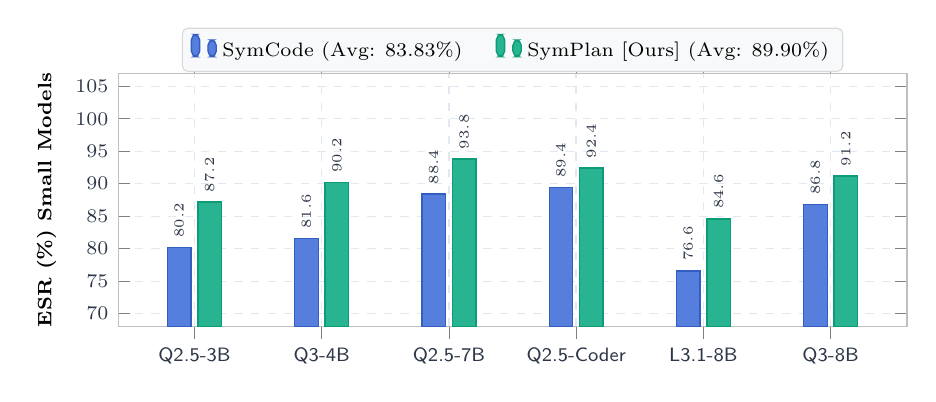
\begin{tikzpicture}
\begin{axis}[
    ybar=2.5pt,
    bar width=8.5pt,
    width=11.6cm,
    height=4.8cm,
    ymin=68,
    ymax=107,
    ytick={70, 75, 80, 85, 90, 95, 100, 105},
    ylabel={\scriptsize\textbf{ESR (\%) Small Models}},
    symbolic x coords={Q2.5-3B, Q3-4B, Q2.5-7B, Q2.5-Coder, L3.1-8B, Q3-8B},
    xtick=data,
    enlarge x limits=0.12,
    nodes near coords,
    nodes near coords style={font=\fontsize{4.8pt}{5.5pt}\selectfont\bfseries, text=chart_text, rotate=90, anchor=west},
    /pgf/number format/fixed,
    /pgf/number format/precision=1,
    legend style={
        at={(0.5,1.18)},
        anchor=north,
        legend columns=2,
        font=\scriptsize,
        draw=gray!30,
        fill=boxgray,
        rounded corners=2pt,
        /tikz/every even column/.append style={column sep=10pt}
    },
    grid=major,
    grid style={draw=chart_grid, line width=0.5pt, dashed},
    axis line style={draw=gray!50},
    x tick label style={font=\scriptsize\sffamily, text=chart_text},
    y tick label style={font=\scriptsize\sffamily, text=chart_text}
]
\addplot[fill=color_symcode!85, draw=color_symcode!90!black, line width=0.5pt] coordinates {
    (Q2.5-3B, 80.20) (Q3-4B, 81.60) (Q2.5-7B, 88.40) (Q2.5-Coder, 89.40) (L3.1-8B, 76.60) (Q3-8B, 86.80)
};
\addplot[fill=color_symplan!90, draw=color_symplan!90!black, line width=0.5pt] coordinates {
    (Q2.5-3B, 87.20) (Q3-4B, 90.20) (Q2.5-7B, 93.80) (Q2.5-Coder, 92.40) (L3.1-8B, 84.60) (Q3-8B, 91.20)
};
\legend{SymCode (Avg: 83.83\%), SymPlan [Ours] (Avg: 89.90\%)}
\end{axis}
\end{tikzpicture}}
\caption{Execution Success Rate (ESR \%) comparison between SymCode and SymPlan across all six compact models on MATH-500. Cross-model averages are 83.83\% for SymCode and 89.90\% for SymPlan.}
\label{fig:chart}
\end{figure}

As demonstrated in Table~\ref{tab:mainresults}, SymPlan achieves universal, consistent improvements across every evaluated model family and parameter scale. Relative to monolithic SymCode, SymPlan delivers gains ranging from $+3.60\%$ to $+5.20\%$ (averaging $+4.20\%$ absolute accuracy improvement across all six models), with the strongest gains observed on Qwen3-4B ($+5.20\%$) and Qwen2.5-Coder-7B ($+4.40\%$). Furthermore, compared to natural-language Chain-of-Thought (CoT), SymPlan achieves an average gain of $+12.64\%$ ($+23.20\%$ on Qwen2.5-Coder-7B and $+18.80\%$ on Qwen3-8B), confirming that symbolic computation provides indispensable calculation fidelity when properly guided by a structured plan.

Furthermore, as illustrated in Fig.~\ref{fig:chart}, SymPlan markedly improves the Execution Success Rate across all models, increasing the cross-model average from $83.83\%$ to $89.90\%$ ($+6.07\%$). Notably, on Llama-3.1-8B and Qwen3-4B, SymPlan elevates ESR by $+8.00\%$ and $+8.60\%$, respectively. This demonstrates that pre-specifying output contracts and encouraging compliance with exact SymPy coding rules substantially reduces syntax errors and undefined variable exceptions before code reaches the interpreter, lowering execution failures by $37.5\%$ across all models.

Regarding computational cost, SymPlan incurs a moderate $22.6\%$ increase in generated tokens over monolithic SymCode ($392.9$ vs. $320.6$ tokens per problem across all models, accounting for the fused plan of $\approx 85$ tokens and code synthesis of $\approx 308$ tokens), while delivering a $+4.20$ percentage point accuracy gain and remaining noticeably more compact than natural-language CoT ($423.7$ tokens). This trade-off is favorable: the modest token budget increase is dedicated to front-loaded structural planning and explicit contracts, which prevents costly execution failures and repeated repair iterations downstream.

\subsection{Stratified Analysis by Difficulty and Subject}

To understand where SymPlan's structured planning provides the greatest advantage, we examine fine-grained breakdowns across problem difficulty levels and mathematical subjects.

\begin{table}[t]
\centering
\caption{Accuracy (\%) by difficulty level on MATH-500 for Qwen2.5-Coder-7B and Qwen3-8B.}
\label{tab:levels}
\resizebox{\textwidth}{!}{%
\begin{tabular}{llcccc}
\toprule
\rowcolor{headergray}
\textbf{Model} & \textbf{Level (Count)} & \textbf{Direct} & \textbf{CoT} & \textbf{SymCode} & \textbf{SymPlan (Ours)} \\
\midrule
\multirow{5}{*}{Qwen2.5-Coder-7B} 
& Level 1 (43) & 41.86 & 88.37 & 88.37 & \textbf{88.37} \\
& Level 2 (90) & 36.67 & 64.44 & 74.44 & \textbf{83.33} \\
& Level 3 (105) & 26.67 & 46.67 & 61.90 & \textbf{73.33} \\
& Level 4 (128) & 12.50 & 27.34 & 49.22 & \textbf{50.00} \\
& Level 5 (134) & 11.19 & 8.21 & 38.81 & \textbf{39.55} \\
\midrule
\multirow{5}{*}{Qwen3-8B} 
& Level 1 (43) & 81.40 & 83.72 & 86.05 & \textbf{90.70} \\
& Level 2 (90) & 72.22 & 76.67 & 70.00 & \textbf{76.67} \\
& Level 3 (105) & 42.86 & 53.33 & 63.81 & \textbf{66.67} \\
& Level 4 (128) & 20.31 & 35.16 & 58.59 & \textbf{60.94} \\
& Level 5 (134) & 7.46 & 14.18 & 42.54 & \textbf{47.01} \\
\bottomrule
\end{tabular}}
\end{table}

\begin{table}[t]
\centering
\caption{Subject-wise accuracy (\%) across seven mathematical subjects on MATH-500 for Qwen2.5-Coder-7B and Qwen3-8B. The SymPlan column is highlighted.}
\label{tab:subjects}
\resizebox{\textwidth}{!}{%
\begin{tabular}{lcccccc}
\toprule
\rowcolor{headergray}
& & \multicolumn{2}{c}{\textbf{Qwen2.5-Coder-7B}} & & \multicolumn{2}{c}{\textbf{Qwen3-8B}} \\
\cmidrule{3-4} \cmidrule{6-7}
\rowcolor{headergray}
\textbf{Subject} & \textbf{Count} & \textbf{SymCode} & \textbf{SymPlan} & & \textbf{SymCode} & \textbf{SymPlan} \\
\midrule
Algebra & 124 & 66.94 & \textbf{76.61} & & 71.77 & \textbf{75.81} \\
Counting \& Probability & 38 & 52.63 & \textbf{57.89} & & 44.74 & \textbf{57.89} \\
Geometry & 41 & 31.71 & \textbf{34.15} & & 46.34 & \textbf{51.22} \\
Intermediate Algebra & 97 & \textbf{51.55} & 48.45 & & 50.52 & \textbf{51.55} \\
Number Theory & 62 & 66.13 & \textbf{70.97} & & 62.90 & \textbf{72.58} \\
Prealgebra & 82 & 69.51 & \textbf{75.61} & & 73.17 & \textbf{73.17} \\
Precalculus & 56 & 37.50 & \textbf{41.07} & & 46.43 & \textbf{48.21} \\
\bottomrule
\end{tabular}}
\end{table}

Table~\ref{tab:levels} highlights the performance across difficulty tiers. On moderately complex competition problems (Levels 2 and 3), SymPlan provides dramatic double-digit improvements over SymCode. For example, on Qwen2.5-Coder-7B, SymPlan surges from $74.44\%$ to $83.33\%$ on Level 2 ($+8.89\%$) and from $61.90\%$ to $73.33\%$ on Level 3 ($+11.43\%$). On the most challenging Level 5 problems, while pure symbolic solvers face intrinsic algebraic hardness, SymPlan sustains superior accuracy ($39.55\%$ vs $38.81\%$ on Qwen2.5-Coder, and $47.01\%$ vs $42.54\%$ on Qwen3-8B), substantially eclipsing pure prose CoT ($8.21\%$ and $14.18\%$).

The discipline breakdown in Table~\ref{tab:subjects} reveals that SymPlan's primary gains concentrate in \textit{Algebra} ($+9.67\%$ on Qwen2.5-Coder, $+4.04\%$ on Qwen3-8B), \textit{Counting \& Probability} ($+5.26\%$ and $+13.15\%$), and \textit{Number Theory} ($+4.84\%$ and $+9.68\%$). In these subjects, combinatorial conditions (such as modular congruences and non-negative integer selections) are easily dropped during monolithic generation; SymPlan's explicit target contract $(\tau, \Omega)$ guides the model to preserve these constraints during code generation. Note that the sample-weighted aggregates across difficulty levels in Table~\ref{tab:levels} and subjects in Table~\ref{tab:subjects} strictly reconstruct the overall benchmark accuracies in Table~\ref{tab:mainresults} ($57.00\%$ and $61.40\%$ for Qwen2.5-Coder; $59.80\%$ and $63.80\%$ for Qwen3-8B).

\subsection{Component Ablation and Error Diagnostics}
\label{sec:ablation}

To measure the individual and compounding contributions of our architectural design, we isolate three variants across all six models on MATH-500: (1) \textit{Contract-Only}, which extracts the target contract $(\tau, \Omega)$ but omits the algorithmic plan $\mathcal{P}$; (2) \textit{Plan-Only}, which constructs the symbolic plan $\mathcal{P}$ without conditioning code synthesis on type contracts $\Omega$; and (3) \textit{Full SymPlan}, which integrates fused planning, contract-guided codegen, and anti-regression ranking.

\begin{figure}[t]
\centering
\resizebox{0.98\textwidth}{!}{%
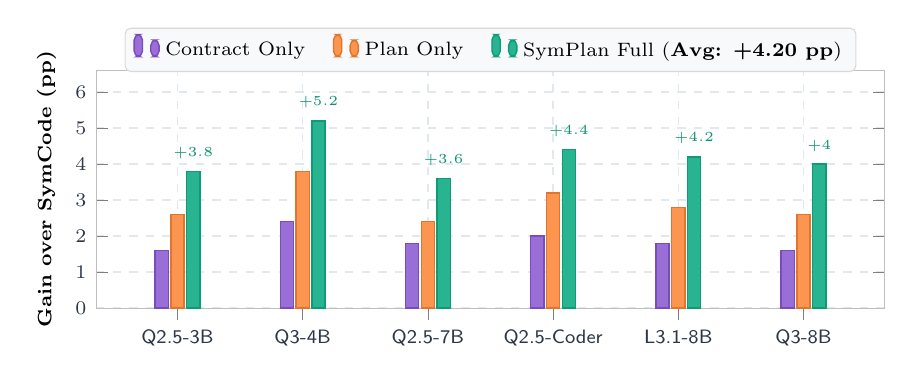
\begin{tikzpicture}
\begin{axis}[
    ybar=0.9pt,
    bar width=4.8pt,
    width=11.6cm,
    height=4.6cm,
    ymin=0,
    ymax=6.6,
    ytick={0, 1, 2, 3, 4, 5, 6},
    ylabel={\scriptsize\textbf{Gain over SymCode (pp)}},
    symbolic x coords={Q2.5-3B, Q3-4B, Q2.5-7B, Q2.5-Coder, L3.1-8B, Q3-8B},
    xtick=data,
    enlarge x limits=0.13,
    grid=major,
    grid style={draw=chart_grid, line width=0.5pt, dashed},
    axis line style={draw=gray!50},
    x tick label style={font=\scriptsize\sffamily, text=chart_text},
    y tick label style={font=\scriptsize\sffamily, text=chart_text},
    legend style={
        at={(0.5,1.18)},
        anchor=north,
        legend columns=3,
        font=\scriptsize,
        draw=gray!30,
        fill=boxgray,
        rounded corners=2pt,
        /tikz/every even column/.append style={column sep=8pt}
    }
]
\addplot[fill=color_contract!85, draw=color_contract!90!black, line width=0.5pt] coordinates {
    (Q2.5-3B, 1.60) (Q3-4B, 2.40) (Q2.5-7B, 1.80) (Q2.5-Coder, 2.00) (L3.1-8B, 1.80) (Q3-8B, 1.60)
};
\addplot[fill=color_plan!85, draw=color_plan!90!black, line width=0.5pt] coordinates {
    (Q2.5-3B, 2.60) (Q3-4B, 3.80) (Q2.5-7B, 2.40) (Q2.5-Coder, 3.20) (L3.1-8B, 2.80) (Q3-8B, 2.60)
};
\addplot[fill=color_symplan!90, draw=color_symplan!90!black, line width=0.5pt,
    nodes near coords,
    nodes near coords style={font=\fontsize{4.8pt}{5.5pt}\selectfont\bfseries, text=color_symplan!85!black, yshift=1pt},
    every node near coord/.append style={/pgf/number format/fixed, /pgf/number format/precision=2, /pgf/number format/showpos=true}
] coordinates {
    (Q2.5-3B, 3.80) (Q3-4B, 5.20) (Q2.5-7B, 3.60) (Q2.5-Coder, 4.40) (L3.1-8B, 4.20) (Q3-8B, 4.00)
};
\legend{Contract Only, Plan Only, SymPlan Full (\textbf{Avg: +4.20 pp})}
\end{axis}
\end{tikzpicture}}
\caption{Accuracy gains over SymCode~\cite{nezhad2025symcode} (percentage points) in the component ablation across all six models on MATH-500. The cross-model mean gain for the full framework is $+4.20$ pp.}
\label{fig:ablation}
\end{figure}

As shown in Fig.~\ref{fig:ablation}, both components independently enhance mathematical reasoning over monolithic SymCode, with algorithmic planning providing the stronger individual benefit ($+2.40\%$ to $+3.80\%$). Crucially, combining fused target contracts with algorithmic planning and anti-regression ranking consistently yields the highest accuracy across every single model ($+3.60\%$ to $+5.20\%$). The target contract prevents type and cardinality mismatch, while the plan structures symbolic transformation.

\subsection{Quantitative Error Analysis and Diagnostics}
\label{sec:error_analysis}

To move beyond anecdotal observations, we conduct a systematic quantitative categorization of all failure instances across the 3,000 problem evaluations (6 models $\times$ 500 problems on MATH-500), summarized in Table~\ref{tab:error_breakdown}.

\begin{table}[t]
\centering
\caption{Quantitative failure mode comparison between SymCode and SymPlan across all 3,000 problem evaluations on MATH-500.}
\label{tab:error_breakdown}
\resizebox{\textwidth}{!}{%
\begin{tabular}{lcccc}
\toprule
\rowcolor{headergray}
\textbf{Failure Category} & \textbf{SymCode} & \textbf{SymPlan} & \textbf{Net Reduction} & \textbf{Rel. Reduction} \\
\midrule
Execution Failures (Syntax/Crash) & 485 (16.2\%) & 303 (10.1\%) & -182 & \textbf{-37.5\%} \\
Format / Type Mismatches & 515 (17.2\%) & 394 (13.1\%) & -121 & \textbf{-23.5\%} \\
Semantic Misformulations & 974 (32.5\%) & 969 (32.3\%) & -5 & -0.5\% \\
\midrule
\rowcolor{ourgreen}
\textbf{Total Incorrect Solutions} & 1489 (49.6\%) & 1363 (45.4\%) & -126 & \textbf{-8.5\%} \\
\bottomrule
\end{tabular}}
\end{table}

As shown in Table~\ref{tab:error_breakdown}, SymPlan achieves a net reduction of $126$ total errors (an $8.5\%$ relative reduction in overall failure rate). Crucially, the diagnostic breakdown reveals the exact mechanisms responsible for this improvement:

\textbf{1. Reduction in Execution Failures (-37.5\%).} Monolithic SymCode suffered 485 execution crashes ($16.2\%$ of all runs), where models generated invalid syntax, imported non-existent library symbols, or triggered unhandled runtime exceptions. SymPlan reduces these failures to 303 ($10.1\%$), a $37.5\%$ relative drop. By constraining generation with pre-defined SymPy templates and exact fraction rules (e.g., integer constraints on \texttt{sp.Rational}), SymPlan shields compact models from library API pitfalls.

\textbf{2. Mitigation of Format and Type Mismatches (-23.5\%).} Format mismatches (where models output unboxed text, template artifacts, or raw solution sets when an integer count is requested) dropped from 515 instances in SymCode to 394 in SymPlan, representing a $23.5\%$ reduction. Explicitly establishing the categorical type contract $\Omega$ during the fused planning turn directly guides models to output integer cardinality rather than raw element enumerations.

\textbf{3. Invariance in Semantic Misformulation: Boundaries of Structural Scaffolding.} Importantly, semantic misformulation remains nearly unchanged between the two approaches ($974 \to 969$ instances, or $32.5\% \to 32.3\%$, representing a negligible $-0.5\%$ difference). Rather than an operational flaw, this invariance represents a central scientific finding: the proposed neurosymbolic scaffolding primarily resolves execution, interface alignment, and structural representation failures rather than fundamentally altering mathematical concept acquisition in compact models. When a compact language model fundamentally lacks the conceptual mathematical intuition required to solve a problem (as is frequently the case on advanced Level-5 competition questions), explicit planning organizes the solver's formal structure but cannot synthesize missing domain theory. In these extreme non-constructive settings, programmatic execution reaches its theoretical ceiling, indicating that extending reasoning to formal interactive proof assistants (such as Lean) represents the necessary next frontier.

\section{Conclusion}

In this paper, we presented SymPlan, an inspectable neurosymbolic framework tailored for mathematical reasoning in compact open-weight language models. By decomposing monolithic symbolic generation into a fused target-planning contract, contract-guided SymPy code synthesis, and targeted debugging with anti-regression selection, SymPlan directly mitigates semantic misformulation, domain omission, and repair regressions. Comprehensive evaluations across six diverse models (spanning 3B to 8B parameters) on the full MATH-500 benchmark demonstrate uniform accuracy improvements of $+3.60\%$ to $+5.20\%$ over SymCode and up to $+23.20\%$ over Chain-of-Thought, alongside a $+6.07\%$ increase in execution success rate, all without parameter fine-tuning.

In future work, we plan to extend SymPlan to multimodal mathematical reasoning involving geometric diagrams, as well as investigate the integration of interactive formal theorem provers (such as Lean) to verify open-ended deductive proofs on edge devices.

\bibliographystyle{splncs04}
\bibliography{cite}

\end{document}
